\begin{frame}{Einführung ins Löten}
    \begin{itemize}\setlength{\itemsep}{3mm}
        \item \begin{center}\textbf{Ziel heute}: sicher löten lernen\end{center}
        \item \begin{center}\textbf{Überblick}: Vortrag mit Sicherheit, Grundlagen und dann Praxis\end{center}
    \end{itemize}
\end{frame}


\begin{frame}{Was nimmst du mit ?}
\begin{itemize}\setlength{\itemsep}{3mm}
  \item 1. Sicherer Umgang mit dem Lötkolben.
  \item 2. Kenntnis der Werkzeuge und Materialien
  \item 3. Gute Lötstellen erkennen
  \item 4. Fehler vermeiden und beheben
\end{itemize}
\end{frame}

\begin{frame}{\textbf{THT} steht für \textit{\textbf{T}hrough \textbf{H}ole \textbf{T}echnology}}
\begin{columns}[T]
    \begin{column}{0.58\textwidth}
        \small
        \begin{itemize}\setlength{\itemsep}{3mm}
            \item Deutsch: \textbf{Durchsteckmontage} oder \textbf{Einsteckmontage}
            \item Die \textbf{Bauteile besitzen Beinchen} und werden durch \textbf{Löcher in der Platine} gesteckt
            \item Die Beinchen werden anschließend auf der \textbf{Rückseite verlötet}
            \item \textbf{Gut geeignet für Einsteiger}, größere Bauteile und \textbf{mechanisch stabile Verbindungen}
        \end{itemize}
        \normalsize
    \end{column}
    \begin{column}{0.42\textwidth}
        \centering
        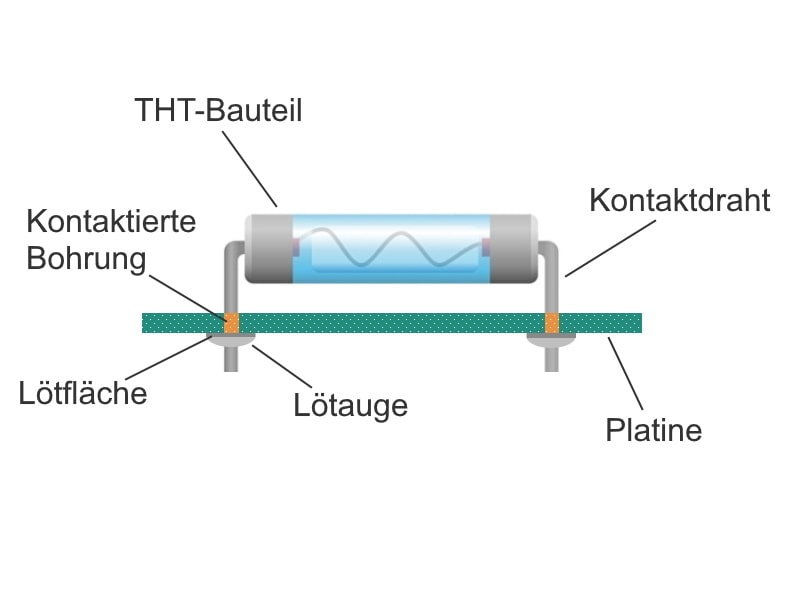
\includegraphics[width=\linewidth,keepaspectratio]{2.0.0.0_content/assets/bilder/tht_löten.jpg}
    \end{column}
\end{columns}
\end{frame}

\begin{frame}{\textbf{SMD / SMT} steht für \textit{\textbf{S}urface \textbf{M}ounted \textbf{D}evice / \textbf{T}echnology}}
\begin{columns}[T]
    \begin{column}{0.58\textwidth}
        \small
        \begin{itemize}\setlength{\itemsep}{3mm}
            \item Deutsch: \textbf{oberflächenmontierte Bauelemente}
            \item Die \textbf{Bauteile werden direkt auf die Oberfläche der Platine} gesetzt
            \item Sie sind meist \textbf{kleiner}, \textbf{kompakter} und oft \textbf{dichter angeordnet}
            \item Sehr verbreitet in \textbf{moderner Elektronik}, aber von Hand meist \textbf{etwas anspruchsvoller zu löten}
        \end{itemize}
        \normalsize
    \end{column}
    \begin{column}{0.42\textwidth}
        \centering
        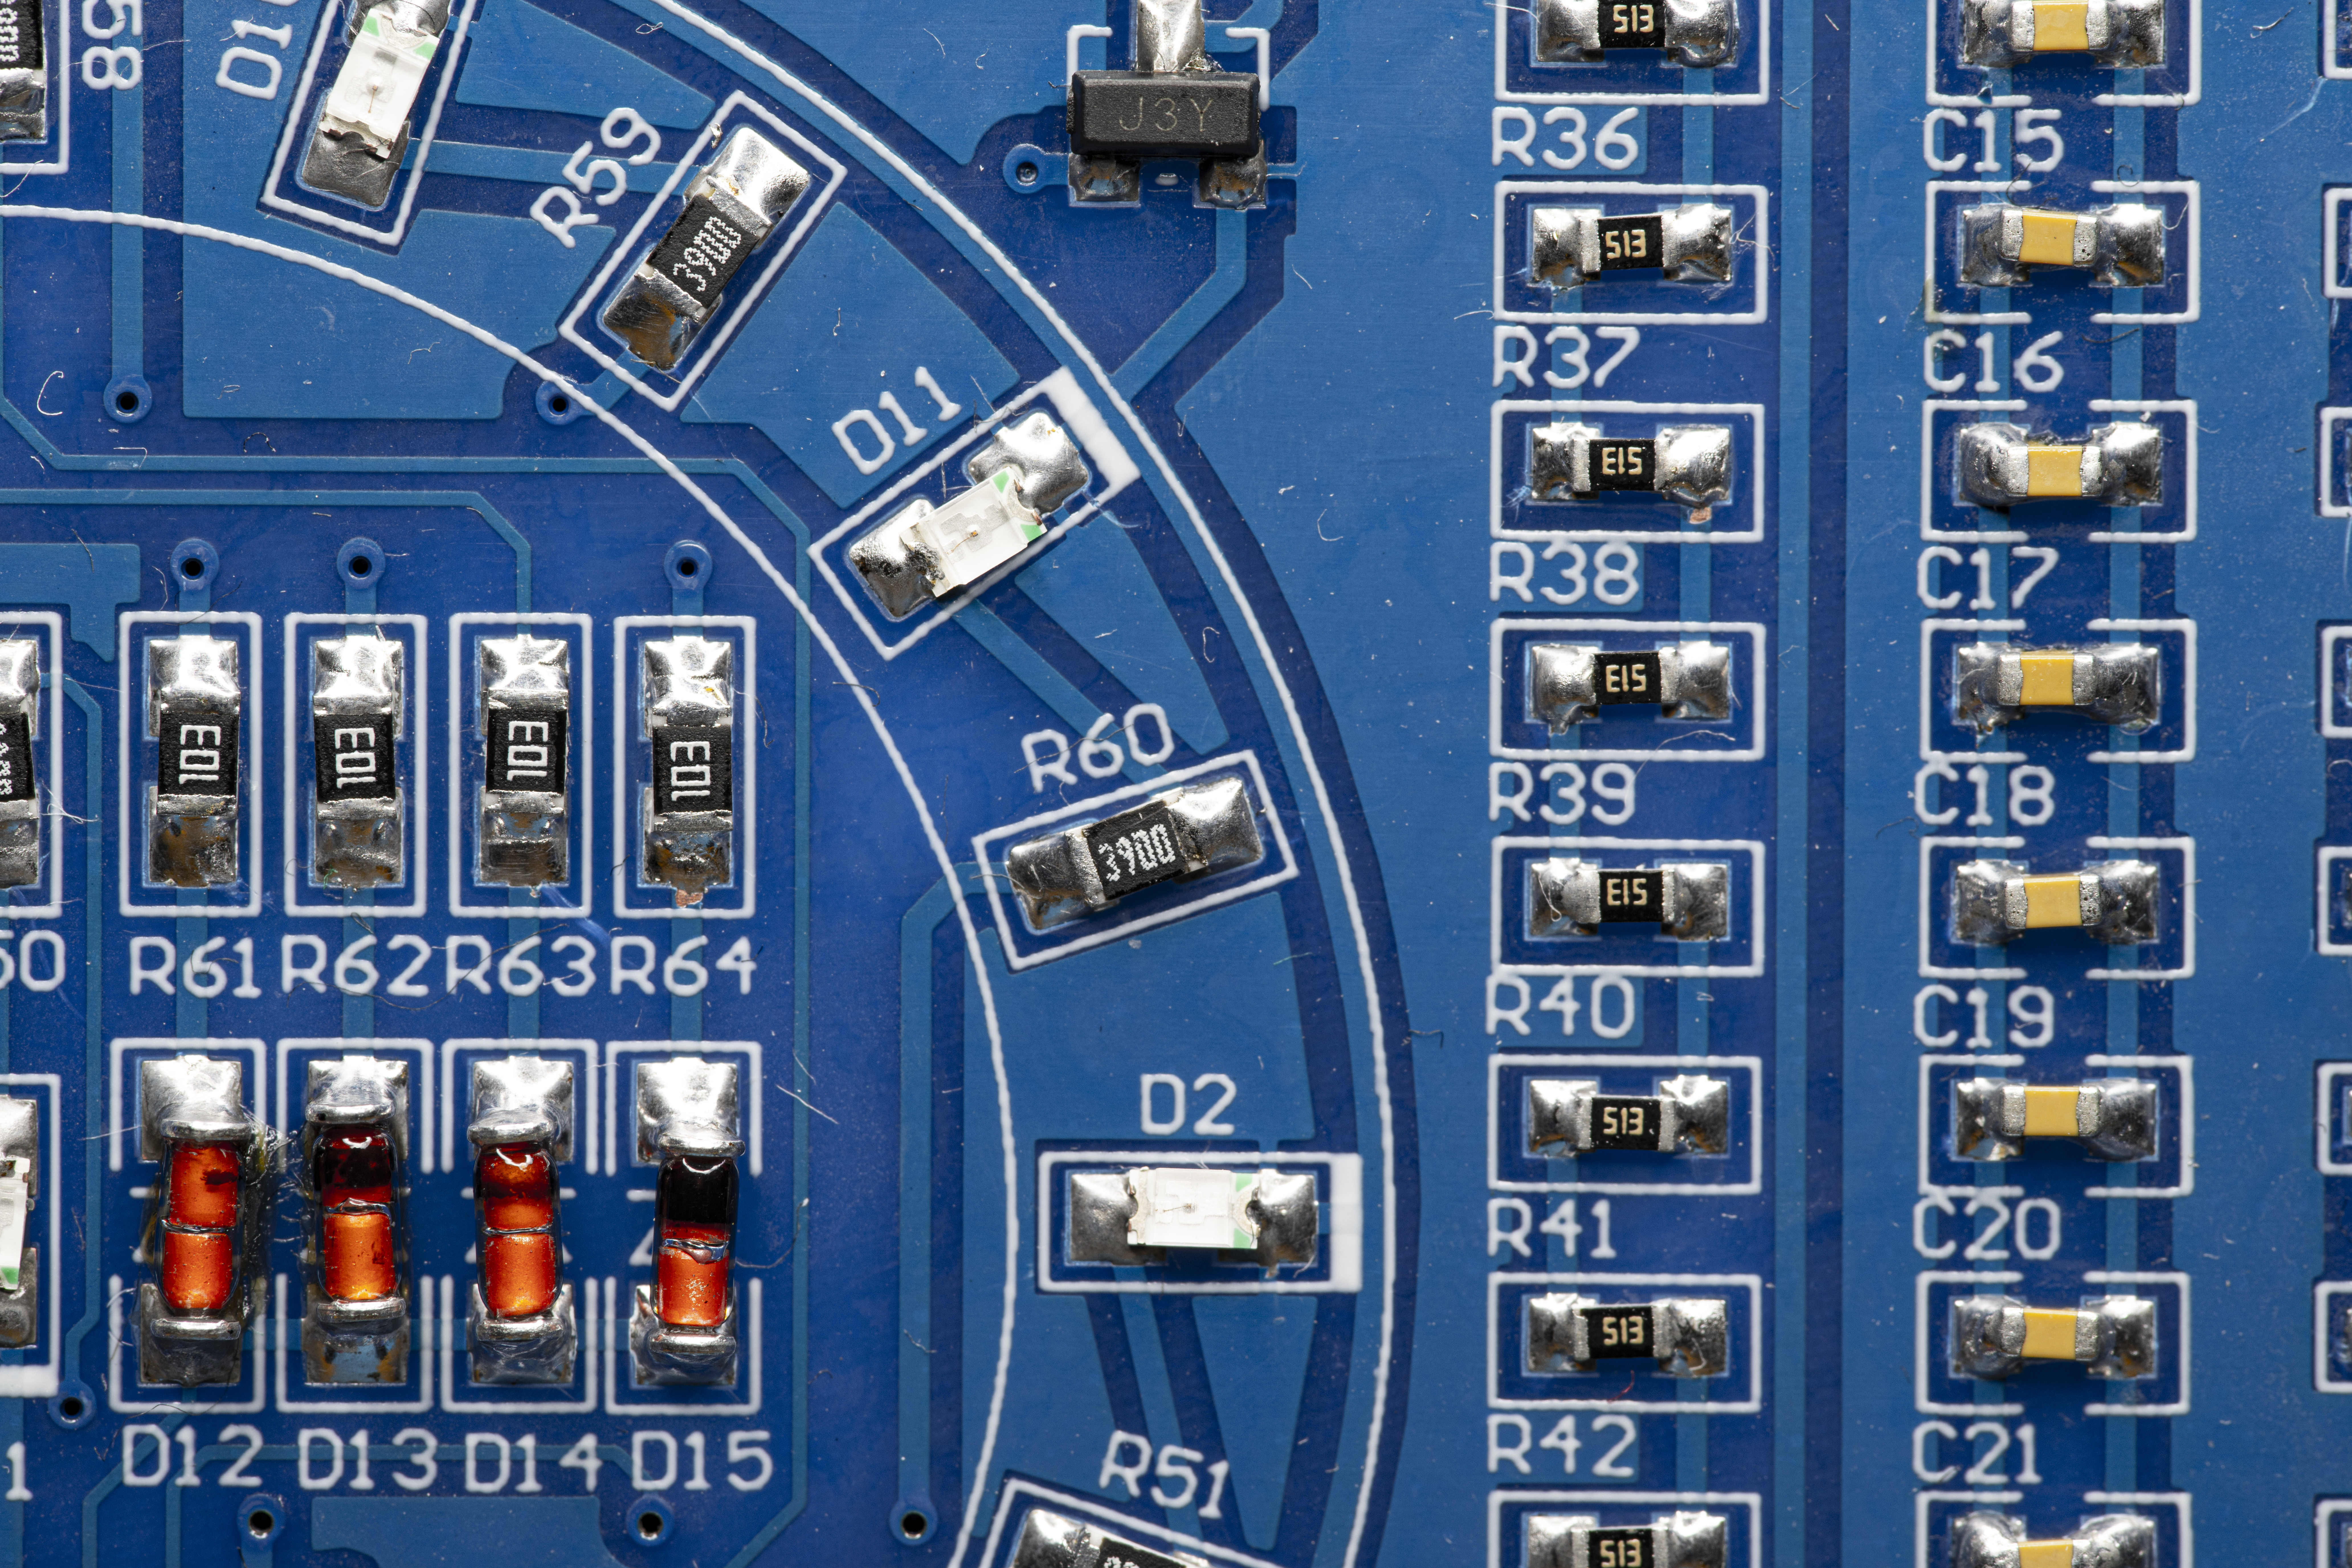
\includegraphics[width=\linewidth,keepaspectratio]{2.0.0.0_content/assets/bilder/smd_löten.jpg}
    \end{column}
\end{columns}
\end{frame}

% Block 3: Wozu und welche Arten
\begin{frame}{Was ist Löten}
\begin{columns}[T]
    \begin{column}{0.58\textwidth}
        \small
        \begin{itemize}\setlength{\itemsep}{3mm}
            \item Beim Löten schmilzt das \textbf{Lot}, die eigentlichen Bauteile bleiben dabei \textbf{fest}.
            \item Dadurch entsteht eine Verbindung, die \textbf{elektrisch leitend} und \textbf{mechanisch belastbar} ist.
            \item In der Elektronik ist das die Grundlage dafür, dass Schaltungen zuverlässig funktionieren.
        \end{itemize}
        \normalsize
    \end{column}
    \begin{column}{0.42\textwidth}
        \centering
        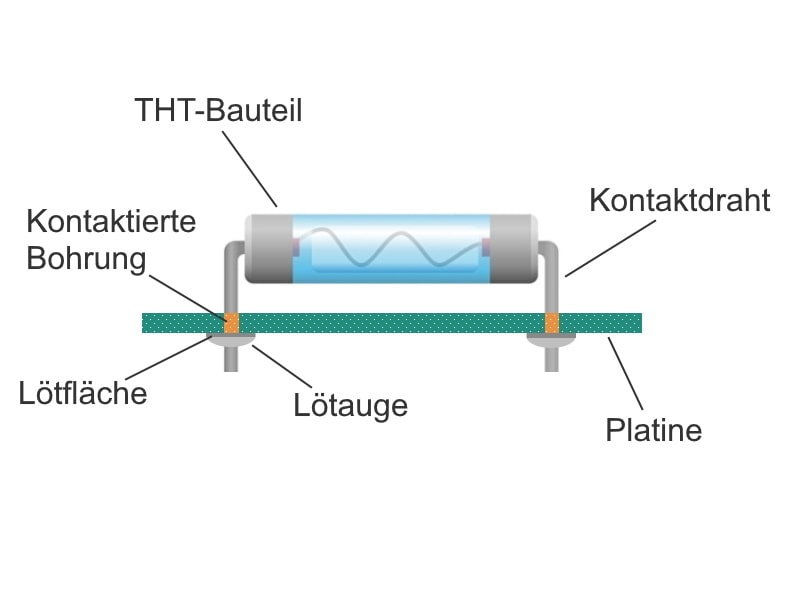
\includegraphics[width=\linewidth,keepaspectratio]{2.0.0.0_content/assets/bilder/tht_löten.jpg}
    \end{column}
\end{columns}
\end{frame}

\begin{frame}{Typische Anwendungen}
\begin{columns}[T]
    \begin{column}{0.58\textwidth}
        \small
        \begin{itemize}\setlength{\itemsep}{3mm}
            \item \textbf{Aufbau von Platinen} und elektronischen Schaltungen
            \item \textbf{Reparatur}, \textbf{Umbau} und \textbf{Modding} von Geräten
            \item \textbf{Maker-Projekte} wie LEDs, Sensoren, Mikrocontroller oder kleine Bausätze
        \end{itemize}
        \normalsize
    \end{column}
    \begin{column}{0.42\textwidth}
        \centering
        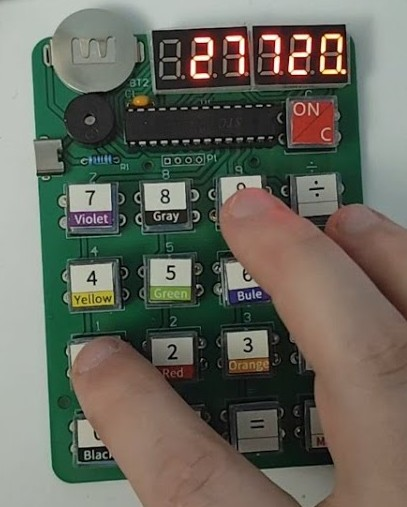
\includegraphics[width=\linewidth,keepaspectratio]{2.0.0.0_content/assets/bilder/projekt_calc_fertig.jpg}
    \end{column}
\end{columns}
\end{frame}

\begin{frame}{Lötarten}
\begin{columns}[T]
    \begin{column}{0.58\textwidth}
        \small
        \begin{itemize}\setlength{\itemsep}{3mm}
            \item \textbf{Weichlöten} wird vor allem in der \textbf{Elektronik} eingesetzt.
            \item \textbf{Hartlöten} kommt eher bei \textbf{Metallbau}, \textbf{Rohrverbindungen} und mechanisch belasteten Teilen vor.
            \item Heute arbeiten wir mit \textbf{Weichlöten}, da es für elektronische Bauteile geeignet ist.
        \end{itemize}
        \normalsize
    \end{column}
    \begin{column}{0.42\textwidth}
        \centering
        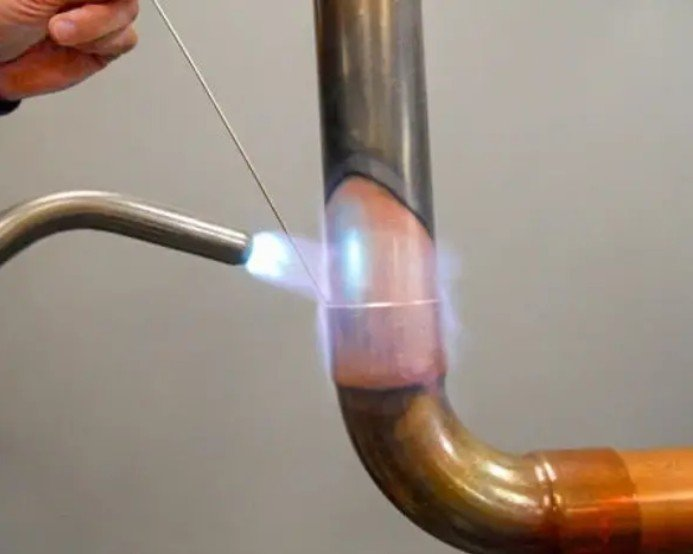
\includegraphics[width=\linewidth,keepaspectratio]{2.0.0.0_content/assets/bilder/hartlöten.jpg}
    \end{column}
\end{columns}
\end{frame}


\begin{frame}{Temperaturrichtlinien}
\begin{columns}[T]
    \begin{column}{0.58\textwidth}
        \small
        \begin{itemize}\setlength{\itemsep}{3mm}
            \item \textbf{THT:} in der Regel \textbf{340\,°C bis 370\,°C}
            \item \textbf{SMD:} bei feinen Pads meist \textbf{320\,°C bis 350\,°C}
            \item Bei \textbf{Masseflächen} oder größeren Kontaktflächen kann kurzzeitig eine etwas höhere Temperatur mit \textbf{Boost} sinnvoll sein
        \end{itemize}
        \normalsize
    \end{column}
    \begin{column}{0.42\textwidth}
        \centering
        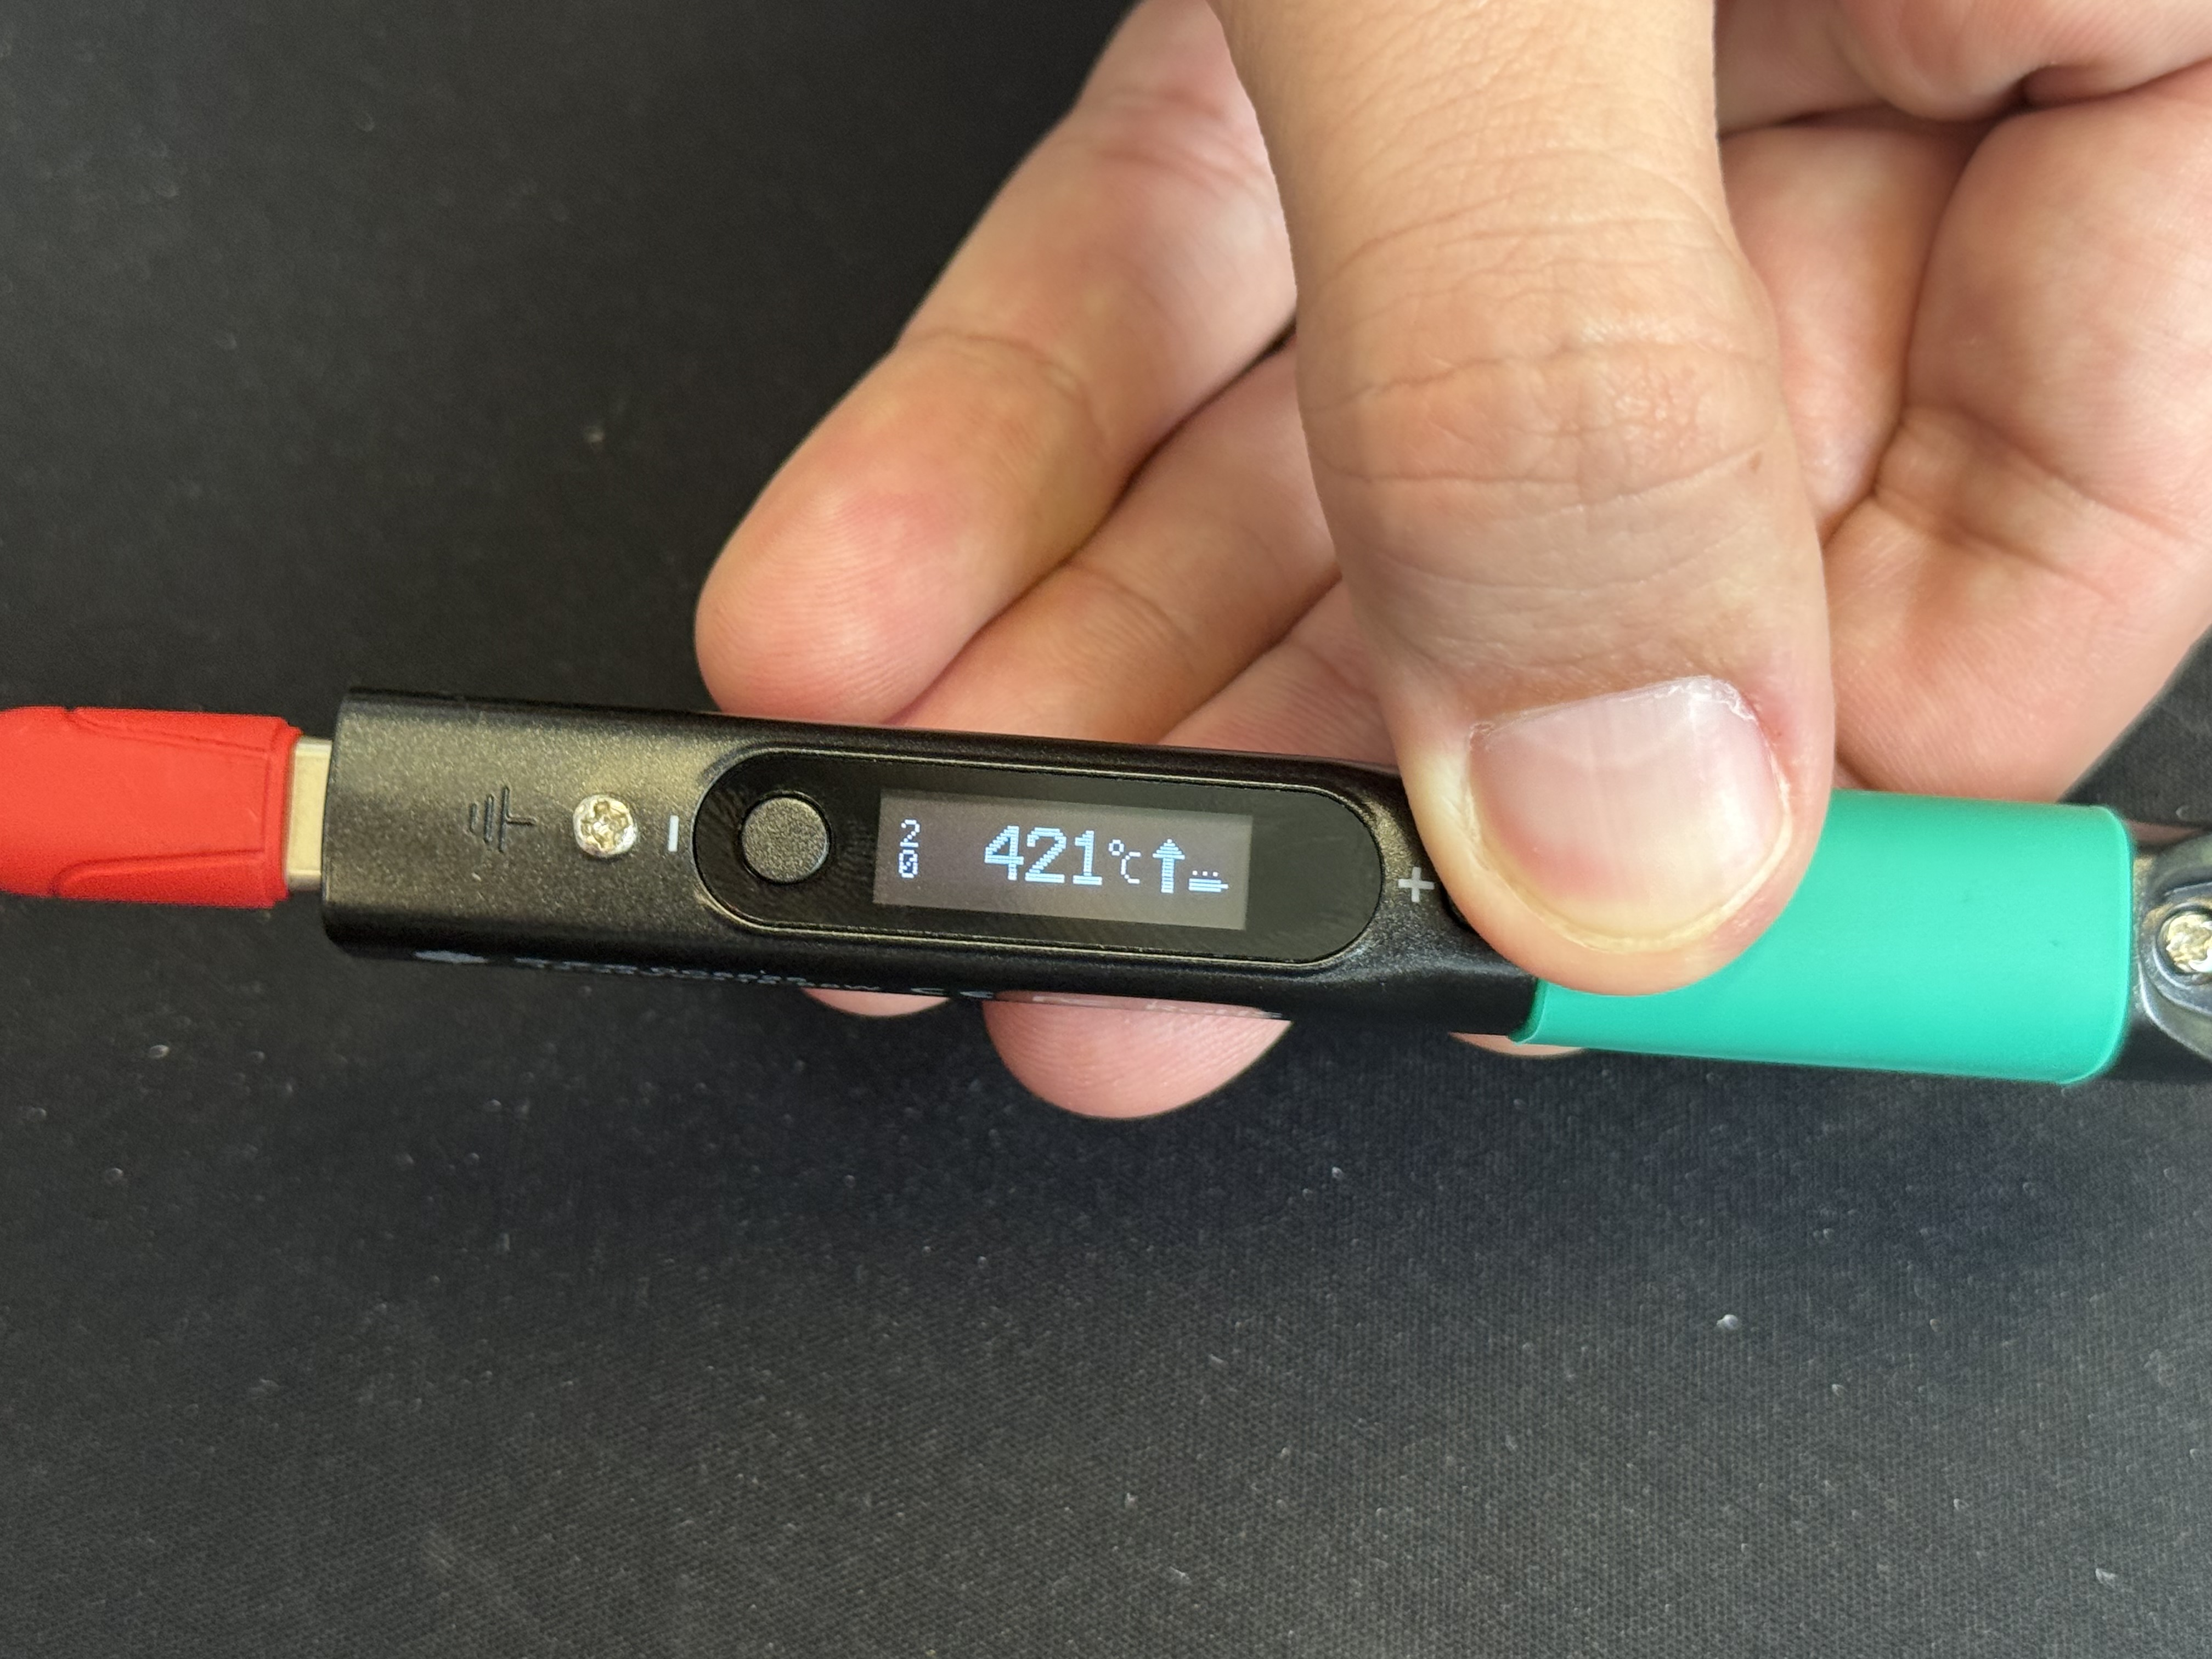
\includegraphics[width=\linewidth,keepaspectratio]{2.0.0.0_content/assets/bilder/lötkolben_Boost.jpeg}
    \end{column}
\end{columns}
\end{frame}

\begin{frame}{Spitzenpflege}
\begin{itemize}\setlength{\itemsep}{3mm}
    \item - Reinigung mit Messingwolle
    \item - Spitze dünn verzinnen
    \item - Feuchter Schwamm optional (haben wir aber nicht)
\end{itemize}
\end{frame}

\begin{frame}{Spitzenaktivator}
\begin{itemize}\setlength{\itemsep}{3mm}
    \item - Aktivator für stumpfe Spitzen
    \item - Sparsam einsetzen
    \item - Danach sofort neu verzinnen
\end{itemize}
\end{frame}